\section{abstract}
% With the emergence of modern web applications, the \emph{Document Object Model} (DOM) of web pages has reached a new level of complexity that prevents the use of state-of-the-art approaches to compare them pairwise.
% Indeed, the existing approaches, like \emph{Tree-Edit Distance} (TED) or \emph{Flexible Tree Matching} (FTM) fail to scale beyond hundred of nodes, which is far below the average complexity of existing web apps.
Tree matching techniques have been investigated in many fields, including web data mining and extraction, as a key component to analyze the content of web pages.
However, when applied to existing web pages, traditional tree matching approaches, covered by algorithms like \emph{Tree-Edit Distance} (TED) or \emph{XyDiff}, either fail to scale beyond a few hundred nodes or exhibit a relatively low accuracy.

%In this article, we therefore propose a novel similarity-based FTM algorithm that proposes a similarity metric to scale beyond the current limits.
In this article, we therefore propose a novel algorithm, named \emph{Similarity-based Flexible Tree Matching} (SFTM), which enables high accuracy tree matching on real-life web pages, with practical computation times.
We approach tree matching as an optimisation problem and leverage node labels and local topology similarity in order to avoid any combinatorial explosion.
Our practical evaluation demonstrates that SFTM significantly improves the state of the art in terms of accuracy, while allowing computation times significantly lower than the most accurate solutions.
By gaining on these two dimensions, SFTM therefore offers an affordable solution to match complex trees in practice.
% Tree Matching consists in computing a node to node matching between two trees. It is an extensively studied problem arising in many different fields. The traditional approach to address this problem is Tree-Edit Distance (TED). TED-based algorithms intend to find the optimal sequence of basic operations to transform a tree into another. TED based algorithms have two main limitations though: 
% \begin{inparaenum}
% 	\item there is currently no TED based algorithm with less than $O(n^3)$ time complexity and
%     \item by definition of TED, once two nodes $n$ and $m$ are matched, descendants of $n$ can only be matched with descendants of $m$ (ancestry restriction), which makes TED a more restrictive problem than general tree-matching.  
% \end{inparaenum}
% A recent work by Kumar et al introduced a novel flexible tree-matching algorithm to relax this ancestry restriction of TED, but the proposed algorithm is impractical to run on trees that have more than a few hundreds of nodes.
% Based on Kumar et al's work, we introduce a novel flexible-tree-matching algorithm that performs in $O(n\ log(n))$ time, thus solving both limitations of TED. In order to do so, we approach tree matching as an optimisation problem and leverage node labels and local topology similarity to avoid combinatorial explosion.
% Finally, we empirically evaluate our algorithm on webpage DOM trees, on both synthetic and real-life examples. Results show that our algorithm qualitatively compares to TED while drastically reducing time complexity.

\section{Introduction} 
% Modern web applications are widely used to assist users in their daily tasks.
The success of Internet has led to the publication and the delivery of a deluge of structured content.
Nowadays, web services and applications are heavily adopting tree-based documents to structure and transfer online content.
However, these web pages keep evolving over time and keeping track of such changes remains a critical issue for the ecosystem and the research community.
Examples of usages that require to detect or track changes in web pages include web extraction~\cite{reis2004automatic,yao2013answer,zhai2005web}, web testing~\cite{choudhary2011water,stocco2017apogen}, comparison of web service versions~\cite{fokaefs2011empirical}, web schema matching~\cite{hao2007web}, and automatic re-organization of websites~\cite{Kumar2011_Bricolage}.

% For example, when it comes to HTML web pages, keeping track of all changes requires to compare \emph{Document Object Model} (DOM) trees across multiples versions of a given resources.
To date, few solutions are specifically designed or tested to match and compare two web pages.
However, the more general question of tree matching has been extensively studied by two families of solutions applicable to the problem of web page matching: 
\begin{inparaenum}
\item \emph{Tree Edit Distance} (TED)~\cite{Tai1979} and TED-related solutions, and
\item XML differentiation (diff) solutions.
\end{inparaenum}

TED is the first and most widely known approach to match trees.
The matchings computed by TED solutions are optimal and there have been much effort into developing openly available efficient implementations of the algorithm~\cite{Pawlik2011,pawlik2015efficient,pawlik2016tree}.
Despite these efforts, TED remains costly to compute. A recent study~\cite{bringmann2018tree} theoretically showed that no algorithm could compute the optimal TED in less than $O(N^3)$ worst time complexity.
To address TED's limitations, several restrictions to TED have been developed. These TED-related algorithms add constraints to the produced matching allowing to trade accuracy for speed.

XML\,diff solutions aim to find the sequence of editions between two XML trees.
The approach is similar to TED, but solutions sometimes make use of XML specificities.
For example, the most widely-known XML\,diff solution---\textsc{XyDiff}~\cite{Cobena2002DetectingDocuments}---is extremely fast, but makes heavy use of XSD schemas and XML primary keys, which cannot be assumed on for any web page.
Without such an additional information, the algorithm unfortunately yields low-accuracy results.

Overall, when matching two web pages, even the most efficient TED implementation~\cite{pawlik2016tree} offers far from optimal accuracy (69\% of precision in average in our empirical evaluation) for computation times often reaching several seconds.
The lack of accuracy may be due to the restrictions TED solutions impose on the produced matching: ancestors and siblings order must be preserved.
However, such restrictions do not hold for web pages and Figure~\ref{fig:ted_mistake} illustrates how TED can report biased matchings, even on simple trees.

\begin{figure}
    \centering
	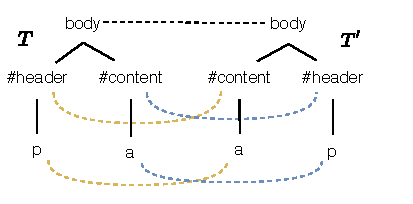
\includegraphics[width=.65\linewidth]{tree-matching/explanation/rted_mistake}
    \caption{Example of matching biased by the TED (as computed by APTED).}
    \label{fig:ted_mistake}
\end{figure}

To address these restrictions when attempting to match two web documents, \cite{fokaefs2011empirical} extended TED with some additional move operations executed \emph{a~posteriori} to address the ancestry restriction and \cite{Kumar2011_FTM,Kumar2011_Bricolage} developed her own \emph{Flexible Tree Matching} (FTM) algorithm to address the ancestry restriction problem.
Unfortunately, while FTM provides a truly restriction-free matching, its high complexity does not allow FTM to scale beyond more than a few dozens of nodes, which is far below the average size of real-life web pages.

% Unfortunately, state-of-the-art algorithms have been proposed to achieve this goal impose to choose between \emph{matching accuracy} or \emph{fast matching}~\cite{xydiff} for any tuple of web documents.
% Furthermore, one can also observe that existing algorithms fail to scale beyond a few hundred of nodes.

% For example, the traditional approach, which is general to any kind of tree, is \emph{Tree Edit Distance} (TED)~\cite{Tai1979} and can be computed in minimum $O(N^3)$ time~\cite{bringmann2018tree}.
% % TED is a restriction of tree matching where descendants of matched nodes can only match with each others (ancestry restriction) and siblings order must be preserved.
% We executed a robust implementation of TED, named APTED~\cite{pawlik2015efficient,pawlik2016tree}, on two instances of the DOM of YouTube, which took more than 4 minutes to propose a matching.
% Unfortunately, when processing and comparing a large dataset of Web documents, one cannot afford such computation times, which makes TED difficult to use in production.

% However, when reproducing this experiment with \textsc{XyDiff},\footnote{\url{https://github.com/fdintino/xydiff}} which is a set of tools for creating and applying deltas from XML documents, results are reported much faster, but the price of a poor accuracy of the resulting tree matchings.

% Figure~\ref{fig:tree_matching_example} illustrates the tree-matching problem. 

% \begin{figure}
%     \centering
% 	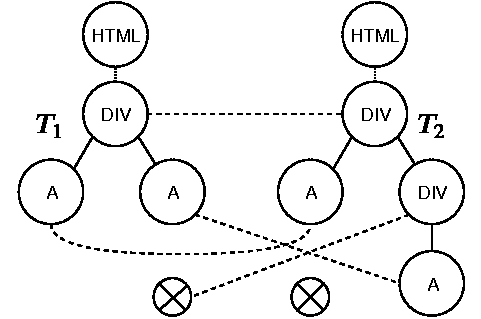
\includegraphics[width=.8\linewidth]{explanation/tree-matching-example}
%     \caption{Example of a tree matching. Crossed circles are auxiliary \emph{no-match} nodes enabling insertions and removals between trees.}
%     \label{fig:tree_matching_example}
% \end{figure}

% The qualitative restrictions or speed limitations of the state of the art therefore led to the development of alternative algorithms.
% For example, \cite{fokaefs2011empirical} extended TED with some additional move operations executed \emph{a~posteriori} to address the ancestry restriction.
% \cite{Kumar2011_FTM,Kumar2011_Bricolage} developed her own \emph{Flexible Tree Matching} (FTM) algorithm to address the ancestry restriction problem, while \cite{reis2004automatic} developed a fast matching system based on top-down matching to extract news faster than TED does. 

In the line of the aforementioned work, this article therefore aims at enabling the fast and non-restricted comparison of complex web pages.
In particular, we propose an alternative to the state-of-the-art FTM algorithm, named \emph{Similarity-based Flexible Tree Matching} (SFTM), that leverages similarity metrics to speed up the comparison of complex trees. 
SFTM shares the properties of FTM to offer a non-restricted tree matching, while offering computation times much lower than FTM, even on restricted versions of the problem.
To match two web page trees, the approach taken by SFTM strongly differs from traditional techniques.
In particular, existing matching algorithms are \textit{structure-centric}: they leverage the structure of both trees to select the nodes to visit and compare.
SFTM instead relies on a \textit{label-centric} approach: it prunes the space of possible matchings using nodes' \emph{label} and considers the tree topology \emph{a~posteriori} to propagate information contained in the nodes.
% Furthermore, our algorithm exposes performance parameters to trade computation time and matching accuracy, depending on applications.
% To the best of our knowledge, SFTM is the first solution to match real-life web documents in practical time (\emph{e.g.}, SFTM matches the DOM of YouTube in less than a second compared to 4 minutes for APTED).
% Through empirical evaluation on real websites, we show that our implementation of SFTM qualitatively compares to APTED and scales in $O(n\cdot log(n))$ with the size of the DOM considered in our experiments, thus making it applicable in many production contexts.

We compared SFTM to other state-of-the-art solutions on a large dataset of popular web pages.
SFTM showed almost twice more efficiency than the best existing solution.
Overall, our algorithm SFTM allows to consistently match real-life web pages with high precision (89\% precision on average) in reasonable time (182\,ms on average).

The code for both SFTM and its benchmark is available openly.\footnote{https://anonymous.4open.science/r/7ae57bd7-3b29-463a-88a4-d31c04ecfcd2/}

The remainder of this article is organized as follows.
Section~\ref{sec:related_work} and~\ref{sec:ftm} cover related work, with section~\ref{sec:ftm} focusing in details on the \emph{Flexible Tree Matching} (FTM) original algorithm.
Section~\ref{sec:SFTM} presents \emph{Similarity-based Flexible Tree Matching} (SFTM), our extension of FTM that leverages the node labels and local topology similarity to guide the comparison.
Section~\ref{sec:evaluation} thoroughly evaluates our solution against the state of the art on a realistic dataset of web documents.
Section~\ref{sec:threats} discusses the threats to validity of our contribution.
Section~\ref{sec:conclusion} concludes and overviews some perspectives for this work.

\section{Related Work}\label{sec:related_work}
% This section overviews the state of the art in the area of tree matching.
\paragraph{\bf \emph{Tree Edit Distance} (TED)}\label{sec:ted}
Comparing two trees is a problem that has been at the center of a significant amount of research.
In 1979, Tai~\cite{Tai1979} introduced the \emph{Tree Edit Distance} (TED) as a generalization of the standard \emph{edit distance} problem applied to strings.
Given two ordered labeled trees $T$ and $T'$, the TED is defined as the minimal amount of node insertion, removal or relabel to transform $T$ into $T'$, while different cost coefficients can be assigned to each type of operation.
By following an optimal sequence of operations applied to $T$, it is possible to match the nodes between $T$ and $T'$.
This problem has been extensively studied since then to reduce the space and time complexity of the algorithm that computes the TED.
To the best of our knowledge, the reference implementation available today is the \emph{All-Path Tree Edit Distance} (APTED)~\cite{Pawlik2011, pawlik2015efficient, pawlik2016tree} with a complexity of $O(n^2)$ in space and $O(n^3)$ in time in the worst case, where $n$ is the total number of nodes ($n = |T_1|+|T_2|$).
In our work, we consider APTED as one of the baselines to evaluate our contribution.

% \subsection{Restrictions of TED}
\cite{bringmann2018tree} showed that TED cannot be computed in worst-case complexity lower than $O(n^3)$.
In order to circumvent this limitation, several restricted versions of the TED problem have been formulated.
The \textit{Constrained Edit Distance}~\cite{zhang1995algorithms, zhang1996constrained} is an edit distance where disjoint subtrees can only be mapped to disjoint subtrees.
The \textit{Tree Alignment Distance}~\cite{jiang1994alignment} is a TED where all insertions must be performed before any deletion.
The \textit{Top-Down} distance~\cite{selkow1977tree} is computable in $O(|T|\times|T'|)$, but imposes as a restriction that the parents of nodes in a mapping must be in the mapping.
The \textit{Bottom-Up} distance~\cite{valiente2001efficient} between trees builds a mapping in linear time, but such mapping must respect the following constraint: if two nodes have been mapped, their respective children must also be part of the mapping.
\cite{reis2004automatic} proposes a variation of the \textit{Top-Down} mapping, called \textit{Restricted Top-Down Mapping} (RTDM), where replacement operations are restricted to the leaves of the trees, which delivers considerable speed gains, despite a theoretical worst case time complexity still in $O(N^2)$.
By definition TED already sets strong restrictions on produced matchings: sibling order and ancestry relationships must be preserved~\cite{zhang1995algorithms}.
These restrictions are particularly problematic when matching two full web pages together~\cite{Kumar2011_Bricolage}.
While above solutions improve computation times, they answer a restricted version of the TED problem leading to an even more restricted set of possible matchings.

\paragraph{\bf XML\,diff}\label{sec:xmldiff}
While TED-related approaches focus on computing a distance between trees, another part of the scientific literature focuses on inferring the set of edit operations between two XML documents.
Most XML\,diff solutions use an intermediary matching step in order to compute the diff.
Computing the set of diff from a given matching is quite straightforward, which means that most works on the subject actually focus on the matching part.
\textsc{XyDiff}~\cite{Cobena2002DetectingDocuments} matches and computes the diff of two XML documents very quickly.
To do so, \textsc{XyDiff} hashes subtrees from both documents and prunes the space of matching possibilities by matching subtrees with identical hashes.
The algorithm can also make use of id attributes and XSD schemas if they exist.
On the other end of the spectrum, \textsc{X-Diff}~\cite{wang2003x} favors accuracy over speed and computes an optimal matching using hashings of path signatures.
\textsc{XKeyDiff}~\cite{dos2007semantical} builds on \textsc{XyDiff} and adds matching logic based on XML primary keys, \texttt{XML\_SIM\_CHANGE}~\cite{viyanon2010xml} and \texttt{XREL\_CHANGE\_SQL}~\cite{sundaram2012change} match XMLs stored in relational databases using SQL. 
\textsc{Phoenix}~\cite{oliveira2018efficient} interestingly uses a more flexible similarity metric between nodes (\emph{e.g.}, to compare the content of two nodes, they use the \emph{Longest Common Sequence}) and choose how to match each subtree by recursively applying the Hungarian algorithm~\cite{kuhn1955hungarian}.
Unfortunately, \textsc{Phoenix} runs in $O(n^4)$ and yields less accurate results than \textsc{X-Diff}.
In our empirical evaluation, we evaluated our solution along with \textsc{XyDiff}, which is widely known and used for XML\,diff, has an efficient implementation openly available and runs in scalable computation times.

\paragraph{\bf \emph{Flexible Tree Matching} (FTM)}
In~\cite{Kumar2011_Bricolage}, TED is found to be unpractical when applied on DOM, as the resulting matching enforces ancestry relationship---\emph{i.e.}, once two nodes $n, n'$ have been matched, the descendants of $n$ can only be matched with the descendants of $n'$, and \emph{vice~versa}. 
Consequently, Kumar~\emph{et~al.}~\cite{Kumar2011_Bricolage, Kumar2011_FTM} introduced the notion of \textit{Flexible Tree Matching} (FTM), which relaxes the ancestry relationship constraint at the price of a stronger complexity.
It restricts its use to small HTML trees composed of less than a hundred nodes, thus making it unpractical for modern web documents, often including more than a thousand nodes.
Furthermore, to the best of our knowledge, there is no public implementation of FTM that can be considered for comparison.

% \subsection{Limitations \& challenges}
We therefore aim at reducing the complexity of the FTM algorithm in order to scale on complex web pages without enforcing restrictions on produced tree-matching solutions.
While all above contributions are structure-based, we build on FTM's approach and rather offer a flexible, label-based matching where labels are used to match nodes and structure is only used \emph{a~posteriori} to improve the matching.

Our contributions therefore read as follows:
\begin{compactenum}
    \item we develop an algorithm inspired by FTM, coined as \emph{Similarity-based Flexible Tree Matching} (SFTM), by leveraging the notion of label similarity, and similarity propagation to reduce the computation time, and
    \item we apply mutations on real-life web documents to provide a thorough evaluation of our implementation of SFTM, showing that it outperforms state-of-the-art approaches in terms of efficiency.
\end{compactenum}

\section{Flexible Tree Matching (FTM)}\label{sec:ftm}
The \emph{Similarity-based Flexible Tree Matching} (SFTM) we introduce in this article can be considered as an extension of the \textit{Flexible Tree Matching} (FTM) algorithm.
This section therefore introduces the FTM algorithm, as originally proposed by Kumar~\emph{et~al.}~\cite{Kumar2011_Bricolage}.
We first describe the notations used throughout the rest of the article, and then describe the main steps of the algorithm.

\subsection{FTM Notations and Overview}
We define an ordered tree $T$ as a directed graph $(N,\prec)$ where $N$ is the non-empty set of nodes and $\prec$ a total order relation that can relate a \emph{child} node $c \in N$ to its \emph{parent} $p \in N$, as $c \prec p$, or \emph{siblings}, as $s \in N$, as $c \prec s$.

In particular, we choose a total order rather than a partial one as the order of siblings has a strong semantic value for a webpage (e.g. the order of paragraphs).

In this article, we always consider \emph{matchings} between two trees $T=(N,\prec)$ and $T'=(N',\prec')$.

Given two trees $T$ and $T'$, the FTM algorithm relies on the complete bipartite graph $G$ between $N^* = N\cup{\Theta}$ and $N'^* = N'\cup{\Theta}'$, where $\Theta$ and $\Theta'$ are \textit{no-match} nodes.
The fact that $G$ is complete means that every nodes of $T^*$ shares exactly one edge with every nodes of $T'^*$.
Formally, we thus have $E(G) = N^* \times N'^*$ where $E(G)$ are the edges of the graph $G$.
An edge $e=(n, n') \in E(G)$ between $n\in N^*$ and $n'\in N'^*$ represents the matching of $n$ with $n'$. Each edge linking a tuple $(n, n')$ is called a \textit{match}.
So, intuitively, $G$ represents all possible matchings between nodes of $T^*$ and $T'^*$ (cf. Figure~\ref{fig:g_SFTM}).

\begin{figure}
    \centering 
    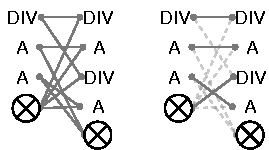
\includegraphics[width=.5\textwidth]{tree-matching/explanation/g_ftm}
    \caption{Building a bipartite graph $G$ representing the set of all possible matchings (left) and then compute the optimal full matching (right).}
    \label{fig:g_SFTM}%
\end{figure}

Formally, we call \textit{matching} and note $M\subset E(G)$, a subset of edges selected from $G$.
A matching $M$ is said to be \textit{full} \emph{iff} each node in $N$ has exactly one edge in $M$ that links it to a node in $N'^*$ and, inversely, each node in $N'$ has exactly one edge in $M$ that links it to a node in $N^*$.
Since matchings need to be \textit{full}, the auxiliary \textit{no-match} nodes $\Theta_1, \Theta_2$ are required to cope with insertion and deletion operations.
The set of possible \textit{full} matchings is restricted to the set of matchings satisfying that every node in $N \cup N'$ is covered by exactly one edge.
\emph{No-match} nodes are the only nodes allowed to be involved in multiple edges.

Given an edge $e=(n, n')\in E(G)$ linking $n$ to $n'$, FTM defines the cost $c(e)$ to quantify how different $n$ and $n'$ are, considering both their labels and the topology of the tree.
Starting from the bipartite graph $G$ describing all possible matchings, the idea behind FTM is to compute the costs $c(e)$ of each edge $e\in E(G)$ and to find the optimal matching with respect to these estimated costs---\emph{i.e.}, to select the set of edges $M\subset E(G)$, such that $M$ is \textit{full} and $c(M)$ is minimal (where $c(M) = \sum_{e\in M}c(e)$).

The upper part of Figure~\ref{fig:steps} describes the main steps involved in computing the final full matching between $T$ and $T'$.

\begin{figure*}
    \centering
	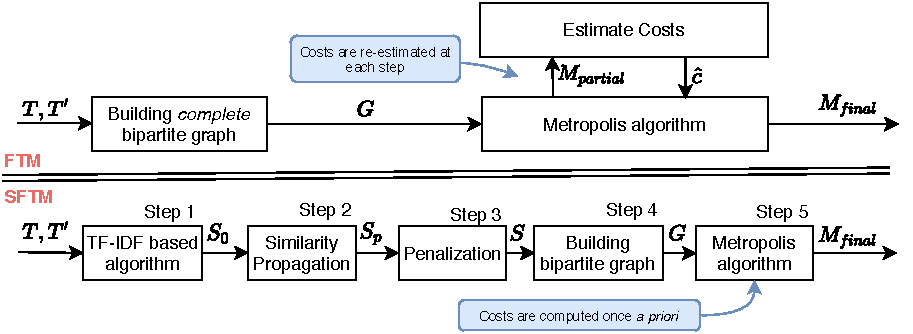
\includegraphics[width=\linewidth]{tree-matching/explanation/ftm-sftm-steps}
    \caption{Steps to compute a full matching between two trees $T$ and $T'$. Upper part covers FTM, while lower part is SFTM.}
    \label{fig:steps}
\end{figure*}

\subsection{Cost Estimation}\label{sec:FTM_cost}
As FTM provides a wide flexibility regarding possible matchings, the design of the cost function $c$ is a key parameter in order to obtain a matching that takes into account both the labels and the topology of the trees.
Typically, the cost $c(e)$ of an edge $e$ between two nodes $n$ and $n'$ is estimated by FTM as follows:
%\text{if }n\text{ or }m\text{ is a no-match node}
\begin{equation}\label{eq:FTM_cost}
c(e) =
\begin{cases}
    w_n                                  & \text{ if}\ n\ or\ n' \in \{\Theta, \Theta'\} \\
    w_r c_r(e) + w_a c_a(e) + w_s c_s(e) & \text{ otherwise}
\end{cases}
\end{equation} 
where $\Theta, \Theta'$ are \textit{no-match} nodes, $w_n$ is the penalty when failing to match one of the edge ends, $c_r(e)$, $c_a(e)$ and $c_s(e)$ are the cost of \textit{relabeling}, \textit{violating ancestry relationship} and \textit{violating sibling group}, respectively, and $w_r$, $w_r$ and $w_r$ their associated weight in the cost function.
$w_n, w_r, c_r, w_a$ and $w_s$ are parameters of the cost function that depend on the kind of matching the user requires.
By extension, we note $c(M) = \sum_{e \in M} c(e)$ the cost of a matching $M$.

Given $e=(n, n')$, the ancestry and sibling costs, $c_a(e)$ and $c_s(e)$, model the changes in topology that matching $n$ with $n'$ entails.
Unfortunately, we can only estimate the costs $c_a$ and $c_s$ if we have access to a full matching, as both costs require a knowledge on how other nodes in the tree were matched (\emph{e.g.}, $c_a$ involves counting the number of children of $n$ matched with nodes that are not children of $n'$).
In order to circumvent the problem, FTM rather considers the approximate costs $\hat{c_a}, \hat{c_s}$ that can be estimated from bounds on the different components of the cost $c$.
Practically, in order to generate one possible full matching, FTM iteratively selects edges in $G$ and, each time an edge is selected, the bounds of $c$ are tightened (we can approximate $c$ more precisely), which means that the costs $\hat{c_a}, \hat{c_s}$ keep being re-estimated along iterations (cf. upper part of Figure~\ref{fig:steps}).
The need to re-estimate the approximated costs after each edge selection actually imposes some critical limitations on the scalability of the algorithm.

\subsection{\textsc{Metropolis} Algorithm}\label{sec:metropolis_ftm}% \cite{Kumar2011_FTM}
Finding the optimal matching, given the graph $G$ and the cost function $c$ is a challenging problem, the authors even proved in~\cite{Kumar2011_FTM} that this problem is NP-hard.
Consequently, the authors described how to use the \textsc{Metropolis} algorithm~\cite{metropolis1953equation} to approximate the optimal matching. 
The \textsc{Metropolis} algorithm provides a way to explore a probability distribution by random walking through samples.
FTM uses this algorithm to random walk through several full matchings, and select the least costly.
The \textsc{Metropolis} algorithm requires to be configured with:
\begin{compactenum}
    \item An initial sample (full matching) $M_0$,
    \item A suggestion function (alternative matching) $M_t \mapsto M_{t+1}$,
    \item An objective function to maximize: $f: M \mapsto \text{quality of } M$,
    \item The number of random walks before returning the best value.
\end{compactenum}

Kumar~\emph{et~al.} defines the objective function $f$ by:
\begin{equation} \label{eq:objective_FTM}
	f_{FTM}(M) = \exp(-\beta\ c(M))
\end{equation}
In order to suggest a matching $M_{t+1}$ from a previously accepted one $M_t$, FTM selects a random number of edges from $M_t$ to keep, sorts remaining edges by increasing costs and iterate through the ordered edges with a probability $\gamma$ to select it.
Once an edge $e = (n,n')$ is selected, all edges connected to $n$ and $n'$ are removed from $G$, and approximate costs need to be re-estimated for all remaining edges, and then sorted so we can select another edge.
The process is repeated until an alternative full matching is obtained.
Therefore, despite using the \textsc{Metropolis} algorithm to reduce the time complexity of the problem, the overall algorithm remains prohibitively costly to compute (cf. Section~\ref{sec:evaluation}), notably due to the continuous re-estimation of the approximated costs at each step of the full matching generation.

\subsection{Complexity Analysis}\label{sec:ftm_complexity}
The original FTM article~\cite{Kumar2011_FTM} does not report on the complexity nor the computation time of the algorithm.
We, therefore, provide an analysis of FTM's theoretical complexity in order to compare it to the one of SFTM (cf. Section~\ref{sec:complexity}).

When discussing complexity, to simplify the notations, we consider the matching of two trees with the same number of nodes and we note $N$ the number of nodes of both trees.

\paragraph{Complete bipartite graph $G$}
Building the complete bipartite graph requires matching each node from $T$ to one node from $T'$, which requires $O(N^2)$ operations. 

\paragraph{\textsc{Metropolis} algorithm}
For each iteration of the \textsc{Metropolis} algorithm, FTM has to suggest a new matching.
In the worst case, the algorithm should choose among all $N^2$ edges.
Each time an edge between $e_1$ and $e_2$ is selected, all other edges connected to $e_1$ and $e_2$ are pruned and remaining costs requires to be re-estimated.
It means that costs have to be re-estimated and sorted for $N^2$ edges, then $(N-1)^2$ edges (after selection and pruning) and so on, until all edges have been selected or pruned.
This implies that the total number of times the costs are re-estimated and sorted is in $O(\sum^N_{n = 0}n^2)$ = $O(N^3)$.
Estimating the cost for a given edge linking $e_1$ and $e_2$ involves counting the number of potential ancestry and sibling violations, which requires going through all edges connected to siblings and children of $e_1$ and $e_2$.
Even if we assume the number of siblings and children is independent from $N$, it still means that estimating the cost of one edge requires $O(N)$ operations.
Thus, in the worst case, the amount of operations required by FTM for each iteration of the \textsc{Metropolis} algorithm is in $O(\sum^N_{n = 0}n^3)$ = $O(N^4)$ (using Faulhaber's Formula).

Overall, the \textsc{Metropolis} step is the one with highest complexity, which means that the complexity of the FTM algorithm is in $O(N^4)$ where $N$ is the number of nodes to match.

% \section{Similarity-based Flexible Tree~Matching}\label{sec:SFTM}
\section{Similarity-based FTM (SFTM)}\label{sec:SFTM}
Based on the above complexity analysis, \emph{Similarity-based Flexible Tree Matching} (SFTM) replaces the cost system of FTM by a similarity-based cost that can be computed once \textit{a~priori} (cf. Figure~\ref{fig:steps}).
This approach drastically improves computation times and rather exposes a parameter that can be tuned to find the desired trade-off between computation time and matching accuracy (cf. Section~\ref{sec:evaluation}).

Given two trees $T=(N,\prec)$ and $T'=(N',\prec')$, SFTM relies on the specification of a \textit{similarity metric} between nodes $n \in N$ and $n' \in N'$.
We compute this similarity metric for all pairs of nodes $(n,n')$ using \emph{i)} inverted indices for labels and \emph{ii)} label propagation and some penalization heuristics for the topology.
We build a bipartite graph $G$ between nodes of $T$ and $T'$ using this similarity metric to compute the costs and apply the Metropolis algorithm to approximate the optimal full matching from $G$.
This new similarity measure allows SFTM to improve the FTM algorithm in two key aspects:
\begin{compactenum}
	\item when building $G$, we do not create all $|N|\times|N'|$ possible edges. We only consider edges linking two nodes with a non-null similarity; and
    \item when generating a full matching, costs do not need to be updated as these costs solely depend on our similarity measure.
\end{compactenum}
In this section, we therefore
\begin{inparaenum}[(a)]
	\item introduce our new similarity metric, and
    \item describe how we leverage it to approximate the optimal full matching.
\end{inparaenum}

\subsection{Overview of Similarity-based Matching}\label{se:newCost}
The similarity metric between nodes $N$ and $N'$ is computed in two main steps:
\begin{inparaenum}
	\item we compute $s_0$, the initial similarity function using only \textit{labels} of the trees individually, and then
    \item we transform $s_0$ to take into account the topology of the tree and compute our final similarity function $s$.
\end{inparaenum}
The computation of $s_0$ leverages inverted index techniques traditionally used to query text in a large document database.
In our case, the documents we query against are $N$, while queries are extracted from $N'$.
Figure~\ref{fig:steps} illustrates the different steps described in this section.

\subsubsection{Initial Similarity (step\,1)}
To compute the initial similarity $s_0$ between $N$ and $N'$ (cf. \textit{step 1} in Figure~\ref{fig:steps}), we independently compare the labels of $N$ and $N'$ using the \emph{Term Frequency-Inverse Document Frequency} (TF-IDF).
The resulting initial node similarity $s_0$ does not take the topology of the trees into account.

In order to take into account relabeling cost between nodes, some existing solutions (\emph{e.g.}, APTED) allow the user to input a pairwise comparison function $label(n), label(m) \mapsto similarity\ score$.
However, computing this similarity score for all the pairs of nodes requires $O(N^2)$ operations.
Thus, to reduce the number of operations, SFTM uses---instead---inverted indices: given a tokenize function $tokenize : n \mapsto \ token\ list$, SFTM
\begin{inparaenum}
	\item decomposes each node $n$ from $N$ into a set of tokens (as defined by the $tokenize$ function), and then
    \item iterates through tokens of nodes $n'$ from $N'$ to increase the value of $s_0(n,n')$ for each token $n$ and $n'$ have in common.
\end{inparaenum}
Section~\ref{tokenSelection} provides a detailed description of the function $tokenize$ we use in our evaluation.

Decomposing nodes from $N$ into tokens allows SFTM to build an inverted index $TM$ (\emph{Token Map}), which maps every token $tk$ with the list of nodes of $N$ that contains $tk$.
The idea behind the inverted index $TM$ is to use the information that a node $n \in N$ contains a token as a differentiating feature of $n$ allowing to quickly compare it to nodes in $N'$.
If a token $tk$ appears in all nodes $N$, this token has no differentiating power.
In general, the rarest a token, the more differentiating it is.
This idea is very common in \emph{Natural Language Processing} (NLP) and a common tool to measure how rare is a token in TF-IDF~\cite{jones1972statistical} and more precisely, the \emph{Inverted Document Frequency} (IDF) part of the formula.
Applying TF-IDF to our similarity yields the following definition:
\begin{align}
	IDF(tk) &= log(|N|/|TM[tk]|) \\
	s_0(n,n') &= \sum_{tk \in TK}IDF(tk)
\end{align}
Where $TK=tokens(n) \cap tokens(n')$.
The function IDF is a measure of how rare a token is, $|TM[tk]|$ is the number of nodes containing the token $tk$ and $tokens$ refers to the user input tokenize function.
Intuitively, we retrieve the tokens shared between nodes $n$ and $n'$ and, for each common token $tk$, we increase $s(n,n')$ by a high value if $tk$ is rare and a low value if $tk$ is common.
In Section~\ref{sec:implementation}, we provide a detailed implementation of how to compute the initial similarity $s_0$.

Tokens that appear in many nodes have little impact on the final score---\emph{i.e.}, low IDF---yet have a very negative impact on the computation time.
In our algorithm, we expose the sublinear threshold function $f: N \mapsto f(N) < N$ as a parameter of the algorithm.
We use $f$ to filter out all the tokens appearing in more than $f(N)$ nodes.
Therefore, $f$ provides a balance between computation time and matching quality: when $N-f(N)$ decreases, computation times and matching quality increase.
In Section~\ref{sec:complexity}, we discuss how $f(N)$ influences the worst-case theoretical complexity.
% An exhaustive theoretical and empirical analysis of precisely how $f$ influences the computation times and matching quality will be the object of future studies.

\subsubsection{Local Topology (step\,2)}
$s_{0}$ represents the similarity between node labels, but does not take into account the topology of the trees.
To weight in local topology similarities, we propagate the score of each node pair to their offspring and siblings.
This idea of propagation is inspired by recent \emph{Graph Convolutional Network} (GCN) techniques~\cite{kipf2016semi}.

The original FTM algorithm includes two terms in the cost function, $c_a$ (ancestry cost) and $c_s$ (sibling cost), which reflect the topology of the trees.
Since we do not use these terms (as they require too much computation time), we need our similarity score to reflect both the similarity of node labels and the similarity of the local topology.
Therefore, we first compute the score matrix $s_0$, based on the label similarity we described above, and then we update this score to take into account the matching score of the parents of $n$ and $n'$.
By doing so, $n$ has a higher similarity score with $n'$ if their respective parents or children are also similar.

Beginning at $s_0$, at each step $i$ and for all pairs that have a non-null initial score  $\{(n, n')\in N \times N' | s_0 \neq 0\}$, we first compute:
\begin{equation}\label{eq:score}
	s_{i}(n, n') \gets s_{i-1}(n, n') +  w_i \times s_{i-1}(p(n), p(n'))
\end{equation}
where $p(n) \in N$ refers to the parent of node $n$.

Similarly, we then increase the score of the parents of $n, n'$:

\begin{equation}\label{eq:score_parent}
	s_{i}(p(n), p(m)) \gets s_{i-1}(p(n), p(n')) +  v_i \times s_{i-1}(n, n')
\end{equation}
where $w_0, w_1\dots w_{P}$ and $v_0, v_1 ... v_P$ are topology weights.
We repeat the process $P$ times ($P$ for propagation) where $P$ is a parameter of SFTM.
The resulting function $s_{P}$ then reflects both label similarity and local topology similarity.

Intuitively, at each iteration, we propagate information further up in the tree.
This is why, the weight sequences $w$ and $v$ should be decreasing so that close kinship among nodes prevails.
From our experiments, we advice the following values for the $P=3$ weights: $w_0 = 0.4, w_1 = 0.04, w_2 = 0.004$ and $w_0 = 0.8, w_1 = 0.08, w_2 = 0.008$.
These values were used and unchanged for all results presented in the empirical evaluation~\ref{sec:evaluation}, leading to high accuracy on a large variety of web documents.

\subsubsection{Penalization (step\,3)}
There are two main drawbacks to the way we propagate the scores in step\,2:
\begin{inparaenum}
\item the scores are still almost exclusively based on labels,
\item nodes with many children may get an unfair score boost from the propagation.
\end{inparaenum}

While (2) can be fixed by normalizing the propagation according to the number of children, the normalization would also potentially remove valuable information.
Instead, for each pair $(n,n')$, we rather apply a penalization proportional to the difference between the number of children of $n$ and $n'$:
\begin{equation}
s(n,n') = s_{P} \times (1 - penalty(n,n'))
\end{equation}
where $penalty(n,n') \mapsto [0, 1]$ is the children penalization defined by:
\begin{equation}
penalty(n,n') = \frac{|(|children(n)|-|children(n')|)|}{max(|children(n)|,|children(n')|)}
\end{equation}
where $|ch(n)|$ is the number of children nodes of $n$.
This step yields the final score function $s$, defined for each couple $(n,n')$.

\subsubsection{Building the bipartite graph $G$ (step\,4)}
Using our final score function $s$, we can now build the bipartite graph $G$: we iterate over all nodes $n \in N$ and we create an edge $e=(n,n')$ for each pair of nodes such that $s_{P}(n,n') \neq 0$ and associate it with the cost $c(n,n') = 1/(1+s_{P}(n,n'))$.
Our resulting cost function is thus defined as follows:
\begin{equation}\label{eq:SFTM_cost}
c_{SFTM}(e) =
\begin{cases}
w_n,                    & \text{if }n\text{ or }n'\text{ is a no-match node}\\
\frac{1}{1+s_{p}(n,n')},& \text{otherwise}
\end{cases}
\end{equation}

Importantly, unlike the bipartite graph built in the FTM algorithm, the resulting bipartite graph $G_{SFTM}$ is \emph{not complete} as only edges, such that $s_{p}(n,n') \neq 0$ are considered.
This is one of the key differences allowing SFTM to drastically improve computation times.

\subsection{Implementation Details}\label{sec:implementation}
In the previous section, we introduced the SFTM algorithm and described how it compares to FTM.
In this section, we describe more precisely how we implement the different steps of SFTM.  

\subsubsection{Node Similarity (step 1, 2 and 3)}
Let us consider two trees $T$ and $T'$.
We first build the dictionary $TM$, an inverted index---\emph{i.e.}, each entry of $TM$ is a tuple $(token, nodes)$ where $token$ is a token (usually a string) and $nodes$ is a \textit{set} of all $n \in N$ that contains $token$.
Figure~\ref{fig:inverted_index} (2a,b) depicts two examples of inverted index.
We note $TM{map}[key]$ the set of $nodes$ whose key in $TM$ is $key$.
In Section~\ref{tokenSelection}, we further describe how we sort HTML nodes into tokens.

\begin{figure*}
    \centering
    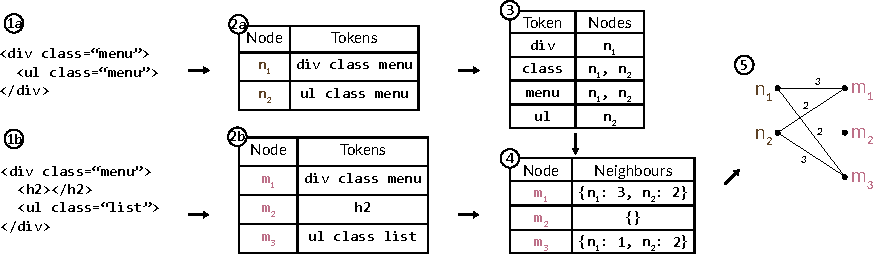
\includegraphics[width=\linewidth]{tree-matching/explanation/inverted_index}
    \caption{Creating the bipartite graph $G$ from two example DOMs $T,T'$. (1a,b)~are the input DOMs, (2a,b)~the extracted tokens, (3)~the inverted index $TM$, (4)~the neighbours dictionaries, and (5)~the resulting bipartite graph $G$. For simplicity, the figure shows a matching where $IDF(tk)=1$, $P=0$ and no-match nodes are not displayed.}\label{fig:inverted_index}
\end{figure*}

Given the inverted index $TM$, we define the function $IDF: tk \mapsto log(|N|/|TM[tk]|)$.
In order to limit the complexity of our algorithm, we remove every token $tk \in TM$ that is contained by more than $f(N)=\sqrt{N}$ nodes, where $f$ is the chosen sub-linear threshold function.
This is equivalent to putting a threshold on $IDF$ to only keep tokens $\{tk \in TM |IDF(tk) > log(\sqrt{N})\}$.
Removing the most common tokens has a limited impact on matching quality, since these are exactly the tokens that provide the least information on the nodes they appear in.

\begin{algorithm}
\SetAlgoLined
\KwIn{\\
n': a node in $N$\\
$TM$: token map, dictionary of nodes from $T$ per token
}
\KwResult{neighbors: a dictionary of scores per node in $T$}
$neighbors \gets new\ Dictionary()$\\
\ForEach{tk in tokens(n')} {
    \ForEach{$n$ in $TM[tk]$} {
        $neighbors[n] += IDF(tk)$\\
    }
}
\Return neighbors
\caption{For a given node $n'\in N'$, compute similarity score $s_0(n,n')$ with all $n\in N$, such that $s_0 > 0$}\label{scoreAlgo}
\end{algorithm}

Once we have the token index $TM$ and the function $IDF$, we apply Algorithm~\ref{scoreAlgo} on each node $n' \in N'$.
In Algorithm~\ref{scoreAlgo}, we first compute the tokens of node $n'$ and, for each token $tk$, we use $TM$ to retrieve the nodes $n \in N$ that contain the token $tk$.
Each node $n$ thus retrieved is considered as a \textit{neighbor} of $n'$---\emph{i.e.}, $s_0(n,n') \neq 0$.
Finally, for each neighbour $n$ of $n'$, we add $IDF(tk)$ to the current score $s_0(n,n')$.
At this point, we have a $neighbors(n')$ dictionary for each node $n' \in N'$.
Each $neighbors(n')$ dictionary contains all non-null matching scores: $\forall n \in keys(neighbors(n')), neighbors(n')[n] = s_0(n,n')$.
Using the Equation~\ref{eq:score}, we can now easily compute $s_{p}$ and $s$.

\subsubsection{Building the Token Vector}\label{tokenSelection}
The actual labels are never directly used by SFTM. The algorithm only leverages the tokens extracted from these labels. The way we choose to extract the tokens contained in a node $n$ thus strongly influences the quality of our similarity score.
% Finding the optimal way to compute these tokens has been the topic of extensive studies~\cite{christen2011survey, steorts2014comparison, datar2004locality}.
We implemented the following function $tokens$ to report all the tokens of a node $n$.
Given $n$, an HTML node representing a \texttt{tag}:
\begin{verbatim}
  <tag att_1="val_1" ... att_2="val_2">
    CONTENT
  </tag> 
\end{verbatim}
where $l$ is the number of attributes, $(att_i, val_i), i \in [1,l]$ are the attribute/value pairs of $n$ and the absolute XPath of $n$ is $xPath(n)$.
We decompose $n$ into the following tokens:
\begin{equation}
	tokens(n) = \{xPath(n), \texttt{tag}, att_1..a_l, tok(val_1)..tok(val_l)\}
\end{equation}
where $tok$ is a standard string tokenizing function that takes a string and splits it into a list of tokens on each non Latin character.
The absolute XPath of a node $n$ in a tree is the full path from the root to the element where ranks of the nodes are indicated when necessary---\emph{e.g.}, \texttt{html/body/div[2]/p}.

SFTM does not include the text content of the nodes in the extracted token vectors.
This decision allow to match pages in different languages or containing different content (e.g. news website) in a robust way.

\subsubsection{Building G (step\,4)}
Using Equation~\ref{eq:SFTM_cost}, we compute the cost $c(n,n')$ for each couple $(n,n')$ where $s_p(n,n') \neq 0$.
Then, for each node $n'\in N'$, we add one edge for all nodes $values(neighbours(n')) \subset N$.

\subsubsection{Metropolis Algorithm (step\,5)}
Once we built the graph $G$ with its associated costs, we need to find the set of edges $M$ in $G$ that represents the best full matching between $T$ and $T'$.
In order to do so, we apply the \textsc{Metropolis} algorithm in a different way than FTM does: 
\begin{inparaenum}
	\item we adopt an alternative objective function, and
    \item SFTM matching suggestion function is faster to compute, as costs never need to be re-estimated.
\end{inparaenum}

Typically, FTM uses the objective function $f_{FTM}(M) = \exp(-\beta\ c(M))$.
In the original FTM article, the authors noted that the parameter $\beta$ seemed to depend on $|M|$.
In order to avoid this dependency, we therefore normalize the total cost:
\begin{equation}
	f_{SFTM}(M) = \exp(-\beta\ \frac{c(M)}{|M|})
\end{equation}
The function $suggestMatching: M_i \mapsto M_{i+1}$ takes a full matching $M_i$ and returns a full matching $M_{i+1}$ related to $M_i$.
In Algorithm~\ref{suggestMatching}, 
\begin{compactenum}
	\item $selectEdgeFrom(edges)$ loops through $edges$ (in order) and, at each iteration $j$, has a probability $\gamma \in [0,1]$ to stop and return $edges[j]$,
    \item $connectedEdges(edge)$, where $edge$ connects $u$ and $v$, returns the set $E$ of all edges connected to $u$ or $v$ (note that $edge \in E$).
\end{compactenum}

\begin{algorithm}
\SetAlgoLined
\KwData{$G$ : The bipartite graph}
\KwIn{$M_i$: A full matching}
\KwResult{$M_{i+1}$: the suggested full matching}
 $M_{i+1} \gets []$  \\
 $remainingEdges \gets sortedEdges(g)$ \\
 $toKeep \gets randomInt(0, |M_i|)$ \\
 \For{j = 0 ... toKeep}{
    edge $\gets$ remainingEdges.first \\
 	$M_{i+1}$.add(edge)\\
    remainingEdges.removeAll(connectedEdges(edge))
 }
 \While{$remainingEdges$ is not empty} {
    $edge \gets selectEdgeFrom(remainingEdges)$ \\
    $M_{i+1}$.add(edge)\\
    remainingEdges.removeAll(connectedEdges(edge))
 }
 \Return $M_{t+1}$
 \caption{Suggest a new matching}\label{suggestMatching}
\end{algorithm}

In practice, we first compute all the connected nodes and edges before storing them as dictionaries, so that the function $connectedEdges$ in Algorithm~\ref{suggestMatching} can be computed in $O(1)$ time.
It is worth noting that, to allow fast removal, the list $remainingEdges$ is implemented as a double-linked list.
The parameter $\gamma$ defines a trade-off between exploration (low $\gamma$) and exploitation (high $\gamma$).
For the Metropolis related parameters, we used mostly the values advised in the original FTM article~\cite{Kumar2011_FTM}: $\gamma = 0.8, \beta = 2.5$ and a number of iterations of 10.

\subsection{Complexity Analysis}\label{sec:complexity}
We are interested in evaluating the time complexity of the algorithm with respect to the size of both trees $N$.
In our analysis, we consider that $N_{tk}=max(|tokens(n)|, n \in nodes(T))$, the maximum number of tokens per node is a constant since it does not evolve with $N$.

When building $G$, we first compute the inverted index $TM$, which requires to iterate through the tokens of all the nodes in $T$, and thus implies a complexity in $O(N \cdot N_{tk}) = O(N)$.

To find the neighbours of nodes from $T'$ using $TM$, we iterate through all the nodes in $T'$, while each node in $T'$ has $N_{tk}$ tokens.
The number of nodes containing a token is artificially limited to $f(N)$.
Thus, building the similarity function $s_0$ takes $O(N \cdot f(N))$ time.

For each node $n'$ in $T'$, we create an edge for each neighbor $n$ of $T$.
Each token $tk \in tokens(n')$ adds up to $f(N)$ neighbors.
It means that the total number of edges is in $O(N \cdot N_{tk} \cdot f(N))$ = $O(N \cdot f(N))$.

Before executing the \textsc{Metropolis} algorithm on $G$, we sort all the edges by cost, which takes $O(N \cdot f(N) \cdot log(N \cdot f(N))) = O(N \cdot f(N) \cdot log(N))$ (as $f(N) \leq N$).
Finally, at each step of the \textsc{Metropolis} algorithm, we run the $suggestMatching$ function, which prunes a maximum of $O(f(N))$ neighbors for each one of the $N$ edges it selects.

Overall, sorting all edges requires the highest theoretical complexity: $O(N \cdot f(N) \cdot log(N))$.
If no threshold is set---\emph{i.e.}, $f(N) = N$---then the worst-case overall complexity of SFTM is $O(N^2 \cdot log(N))$, which keeps outperforming TED ($O(N^3)$) and FTM ($O(N^4)$).

In this evaluation, we used $f(N) = \sqrt{N}$, which leads to a theoretical worst-case complexity in $O(N \cdot \sqrt{N} \cdot log(N))$.
% The empirical evaluation conducted in Section~\ref{sec:evaluation} tends to suggest that the average-case complexity may be even lower in practice.

\section{Empirical Evaluation}\label{sec:evaluation}
The objective of this evaluation is to assess that:
\begin{compactenum}
	\item the quality of the matchings reported by SFTM compares with the baselines we selected---APTED and \textsc{XyDiff}---and
    \item SFTM offers practical computation times on real-life web pages.
\end{compactenum}

\subsection{Input Web Document Dataset}
We need to assess the ability of SFTM to match the nodes between two slightly different web pages $d$ and $d'$.
To measure and compare the accuracy of all studied solutions, we must have access to the ground truth matching between $d$ and $d'$---\emph{i.e.}, for each node $n$ in $d$, what is the true matching node $n'$ in $d'$.

To the best of our knowledge, there is no established and public benchmark that include such pairs of trees, along with the ground truth matching of their nodes. Creating such a benchmark is challenging.
Existing matching solutions usually do not provide any qualitative empirical benchmark~\cite{Bunke1998ASubgraph,Dinitz1998OnIsomorphism, jiang1994alignment,valiente2001efficient,Wang2001FindingHierarchy,zhang1995algorithms} and challenging matching problems involve thousands of nodes, which makes manual labeling error prone for humans (both trees could not even be rendered on the same screen).
Therefore, we built a a semi-synthetic dataset built from mutations applied to real-life web pages, thus obtaining a large-scale dataset in which the ground truth is known.

\paragraph{DOM mutation}
To build a grounded dataset of $(d,d')$ pairs---\emph{i.e.}, where the ground truth (perfect matching) is known---we developed a mutation-based tool that operates as follows:
\begin{compactenum}
	\item we construct the DOM $d$ from an input web document,
    \item for each element of $d$, we generate a unique signature attribute,
    \item for each original DOM $d$, we randomly generate a set of mutated versions: the \textit{mutants}.
    Each \textit{mutant} $d'$ is stored along with the precisely described set of mutations that was applied to $d$ to obtain $d'$.
    Importantly, the signature tags of the elements in $d$ are transferred to $d'$, which constitutes the perfect matching between $d$ and $d'$. These signatures are obviously ignored when applying the matching algorithms.
\end{compactenum}

In our tool, most attention has been dedicated to the choice of relevant mutations to apply.
We therefore relied on the expertise of web developers to identify the most common changes that can apply to DOM.
Their feedback led to the identification of the following list of mutation operations:
% \begin{center}
%   \begin{tabular}{|l l|} 
%       \hline
%       Element       & Mutation operators\\
%       \hline
%       \hline
%       \em Structure & \tt remove, duplicate  wrap, unwrap, swap \\
%       \em Attribute & \tt remove, remove words \\
%       \em Content   & \tt replace with random text, change letters, \\
%                      & \tt remove, remove words \\
%       \hline
%   \end{tabular}
% \end{center}

\begin{center}
    \begin{table}[h]
    \begin{tabular}{l|l}
    \hline
    Category  & Mutation Operators                       \\ \hline
    Structure & \tt Remove, duplicate, wrap, unwrap, swap    \\
    Attribute & \tt Remove, remove words                     \\
    Content   & \tt Replace, remove, remove words, change letters \\ \hline
    \end{tabular}
    \end{table}
\end{center}
where
\textit{Structure: remove} removes an element and its children (recursively), 
\textit{duplicate} duplicates a subtree, applies $mutate$ to duplicated subtree and insert the subtree anywhere in the tree,
\textit{wrap} wraps an element within a new $div$ container,
\textit{unwrap} removes an element $e$ and attach the children of $e$ to the parent of $e$,
\textit{swap} swaps the position of two sibling elements,
\textit{Attribute: remove} removes an attribute with its value,
\textit{Attribute: remove words} removes a random number of tokens from the value of an attribute,
\textit{Content: replace} replaces the content of an element with a random text whose size is close to the original,
\textit{Content: change letters} replaces a few letters in the content of an element,
\textit{Content: remove} removes the content of an element,
\textit{Content: remove words} removes random tokens from the content of an element.

We believe that the above mutations are representative of a wide range of changes that apply in web pages, although they may not perfectly cover all the cases encountered in practice.
In particular, the distribution of these mutations might not be uniform in real life---\emph{i.e.} some mutations might happen more than others.
Yet, this evaluation intends to compare the sensitivity of studied matching algorithms to common mutations, which remains a relevant context to estimate and compare their quality.

\paragraph{Input document sample}
We fed our mutation tool with the home pages of the Top\,1K Alexa websites.\footnote{https://www.alexa.com/topsites}
Alexa provides a list of websites ordered by popularity, thus providing a representative list of web pages of variable complexities.
For each original DOM $d$, we created $10$ mutants $d'_0\dots d'_9$ with a ratio of mutated nodes ranging from $0$ to $50\%$ of the total number of nodes on the page, $|nodes(d)|$.

Overall, we obtained a dataset composed of $6,276$ document pairs $d,d'_n$ that could be correctly processed by the algorithms under study.
Figure~\ref{fig:distribution} reports on the size distribution, in number of nodes, of original and mutated web documents included in this dataset.

\begin{figure}
    \centering
    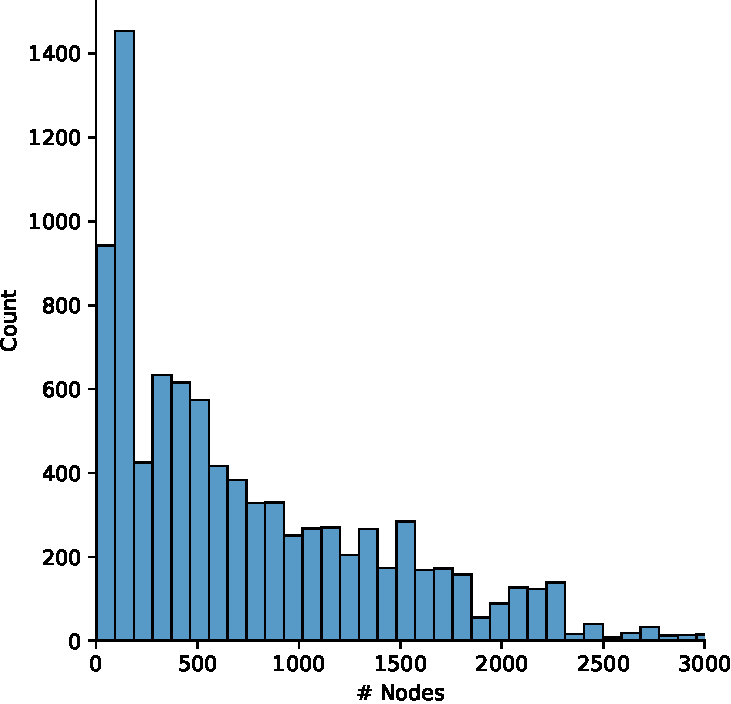
\includegraphics[width=.6\linewidth]{tree-matching/graphs/distribution_size}
    \caption{Distribution of DOM sizes (in terms of nodes) in the dataset.}
    \label{fig:distribution}
\end{figure}

\subsection{Baseline algorithms}
Given no implementation of the original FTM algorithm is available, we implemented and evaluated it, but the computation times and space complexity of this implementation were too high to run the algorithm on real-life web documents (\emph{e.g.} for a tree of 58 nodes, the computation took 1 hour).

We thus mainly compare SFTM to APTED and \textsc{XyDiff}.
APTED is the reference implementation of TED that reports on the best performance so far.
The implementation of APTED used for this evaluation is the one provided by the authors of~\cite{pawlik2016tree,pawlik2015efficient}.
Since APTED yields the optimal solution to the TED problem, TED is theoretically superior in accuracy to all more restricted solutions (see Section~\ref{sec:related_work}).

\textsc{XyDiff} is the most widely-known and used algorithm to efficiently match XML documents. Unlike APTED, XyDiff does not return an optimal result, it instead focuses on speed which makes it a complementary candidate to APTED as a baseline. 
In order to use \textsc{XyDiff} on HTML pages we had to convert the HTML into XHTML, which mostly means closing unclosed tags (\emph{e.g.}, input tags).
We used an existing open source implementation of \textsc{XyDiff}.\footnote{https://github.com/fdintino/xydiff}
We consider the pairs $(d,d')$ taken from the above input dataset, and we systematically ran SFTM, APTED, and \textsc{XyDiff} algorithms with each pair to match $d$ with $d'$ on the same machine.

\paragraph{Ground truth}
When building the dataset, we keep track of nodes' signature so that we always know which nodes from $d$ should match with nodes from $d'$.
This ground truth is hidden from the evaluated algorithms, but is used \emph{a~posteriori} to measure and compare the quality of the matchings computed by the algorithms under evaluation.
% Our purpose in this section is not to conduct a thorough qualitative comparison of the algorithms, since it would require optimizing the parameters of both algorithms in an unbiased way.
% Instead, we show that SFTM returns qualitatively comparable results, while drastically reducing computation time.

\subsection{Experimental Results}\label{sec:performances}
All the results in this section have been obtained by running all three algorithms on the same server containing 252\,GB of RAM and an Intel(R)~Xeon(R) CPU E5-2660\,v3 @ 2.60\,GHz.

\paragraph{Matching quality}
The signature tags injected in nodes from $d$ and $d'$ allow us to assess the quality of the matchings by comparing to the ideal matching $M_{ideal}$.
For the qualitative analysis, we model the tree matching algorithm as a binary classification problem: Given two trees $T$ and $T'$ containing the set of nodes $N$ and $N'$ respectively, $N \times N'$ is the set of all possible matches.
We consider the matching $M_a \subset N \times N'$ produced by a tree matching solution $a$.
Then, a match $e=(n,n') \in M$ is classified as positive by $a$ if $e \in M_a$.
All matches that should be positive are in the ideal matching $M_{ideal}$.
All possibilities are summarized in the following confusion matrix:
\begin{center}
    \begin{tabular}[h]{l|c|c|}
    % \hline
    \cline{2-3} 
    
                                          & $e \in M_{ideal}$ & $e \notin M_{ideal}$ \\
    % \cline{2-3}
    % \cline{1-3}
    \hline
    \multicolumn{1}{|l|}{$e \in M_a$}    & \textbf{True Positive} & False Positive\\
    \hline
    \multicolumn{1}{|l|}{$e \notin M_a$} &         False Positive & \textbf{True Negative}\\
    \hline
    \end{tabular}
    % \caption{Confusion matrix modeling the evaluation of SFTM as a binary classification problem}
\end{center}

Using the above confusion matrix, we can compute the \textit{precision}, \textit{recall}, metrics and the \textit{F1 score}, which are very commonly considered for binary classification problems.

Figure~\ref{fig:f1score} reports on the precision, recall and F1 score of the 3 tree matching solutions we compared, namely SFTM, APTED, and \textsc{XyDiff}.
As expected, the accuracy of all solutions decreases when the mutation ratio increases.
However, for all the reported metrics, SFTM clearly outperforms both \textsc{XyDiff} and APTED.
For both APTED and \textsc{XyDiff}, we believe the lack of accuracy stems from the lack of flexibility when matching labels.
\textsc{XyDiff} relies entirely on hashing subtrees of the document and match subtrees with identical hash.
While this approach might be robust to small structural mutations, it is naturally very sensitive to large amounts of mutations when both structures and labels are mutated.
Similarly, TED compares the labels of most pairs of nodes and generate an associated cost of \texttt{1} when the labels are identical and \texttt{0} when they are different (no gradual costs if the labels are similar).
% We modified the cost function on APTED to provide a more flexible label cost function.
% The accuracy obtained was better (equivalent to SFTM) but the computation times were prohibitive (4 minutes to match youtube pages) which is understandable since this comparison function runs $O(n^3)$ times.
% For this reason, we could only run the modified version of APTED on a few hundred small pages and the results presented in Figure~\ref{fig:f1score} reports on the non-modified version.

\begin{figure}
  \centering
  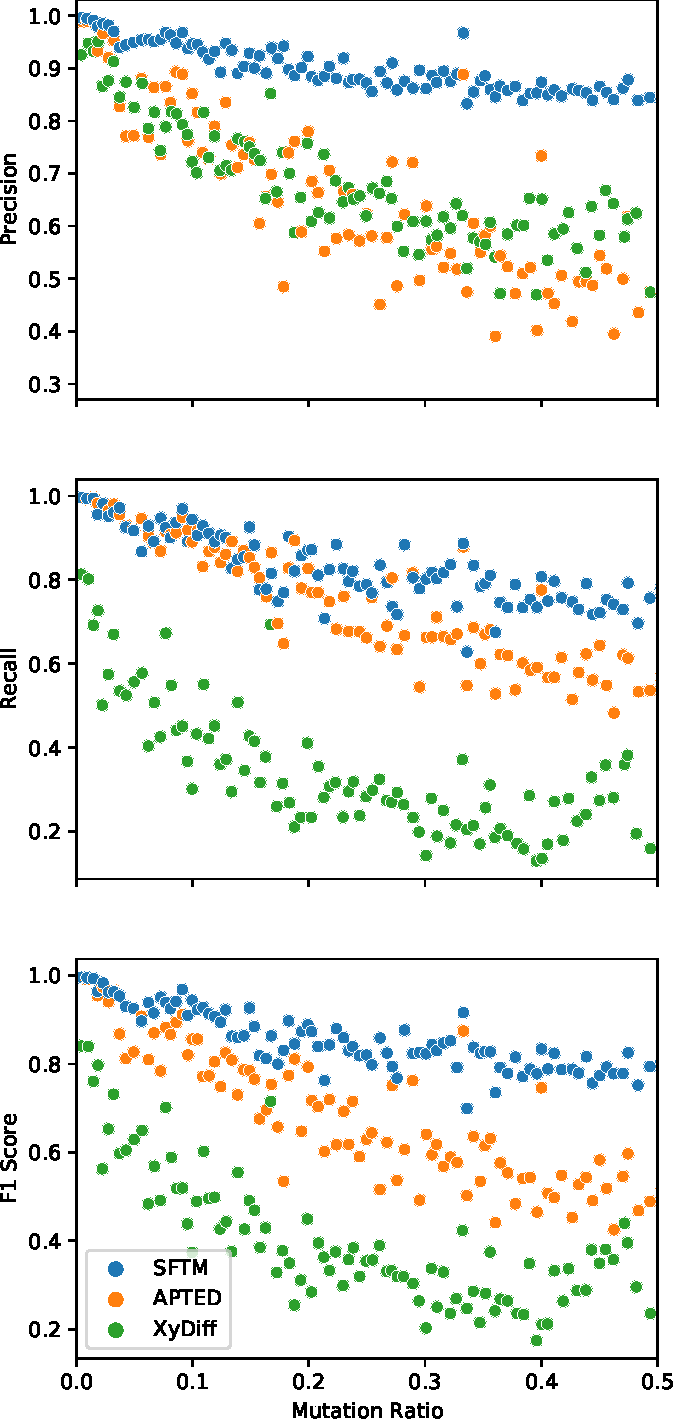
\includegraphics[width=.65\linewidth]{tree-matching/graphs/f1score}
  \caption{Precision, Recall, and F1 Score of SFTM, APTED, and \textsc{XyDiff}.}
  \label{fig:f1score}
\end{figure}

\paragraph{Completion time}
For each couple ($d$, $d'$) retrieved from the dataset, we measured the time taken by SFTM, APTED, and \textsc{XyDiff} to compute a full matching.
Figure~\ref{fig:computation_time} reports on the average time to match DOM couples of increasing size (in terms of number of nodes) for all three solutions.
\textsc{XyDiff} exhibits very fast computation speed and despite its numerous optimizations, APTED's computation times increases exponentially large web documents.
SFTM is not as fast as \textsc{XyDiff}, but seems to show reasonable growth when the size of web documents increases.
Interestingly, APTED computation time varies greatly, which is due to the multiple heuristics used by this implementation to optimize the computation in certain situations.

\begin{figure}%{\textwidth}
    \centering
    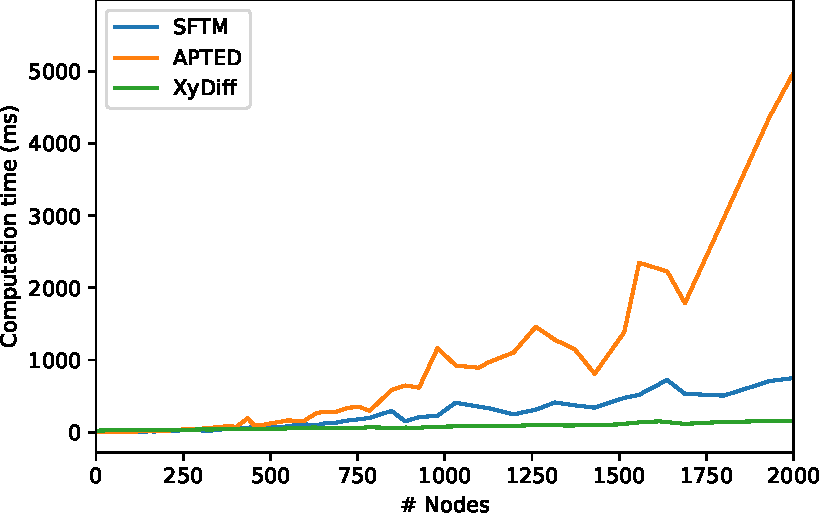
\includegraphics[width=.85\linewidth]{tree-matching/graphs/computationTime}
    \caption{Computation times when matching trees of different sizes.}
    \label{fig:computation_time}
\end{figure}%

Overall, one can observe that SFTM offers an interesting trade-off between two classes of tree matching algorithms: the ones maximizing accuracy at the cost of time, like APTED, and those minimizing the completion time at the cost of reduced accuracy, like \textsc{XyDiff}.

% Figure~\ref{fig:sftm_speed} delivers a closer look on the scalability of SFTM.
% The empirical results seem to indicate an evolution in $O(n \cdot log(n))$: in  Figure~\ref{fig:sftm_speed}, we replaced the X axis from the number of nodes in the DOM $n$ to $n\ log(n)$ then computed a linear regression on the curve which resulted in a correlation coefficient $r^2 = 86\%$.
% We believe the complexity depends on the distribution of nodes within the tokens and a more thorough theoretical analysis will be conducted in the future to understand the gap with the theoretical complexity (cf. Section~\ref{sec:complexity}). 

    % \begin{figure}%{\textwidth}
    %     \centering
    %     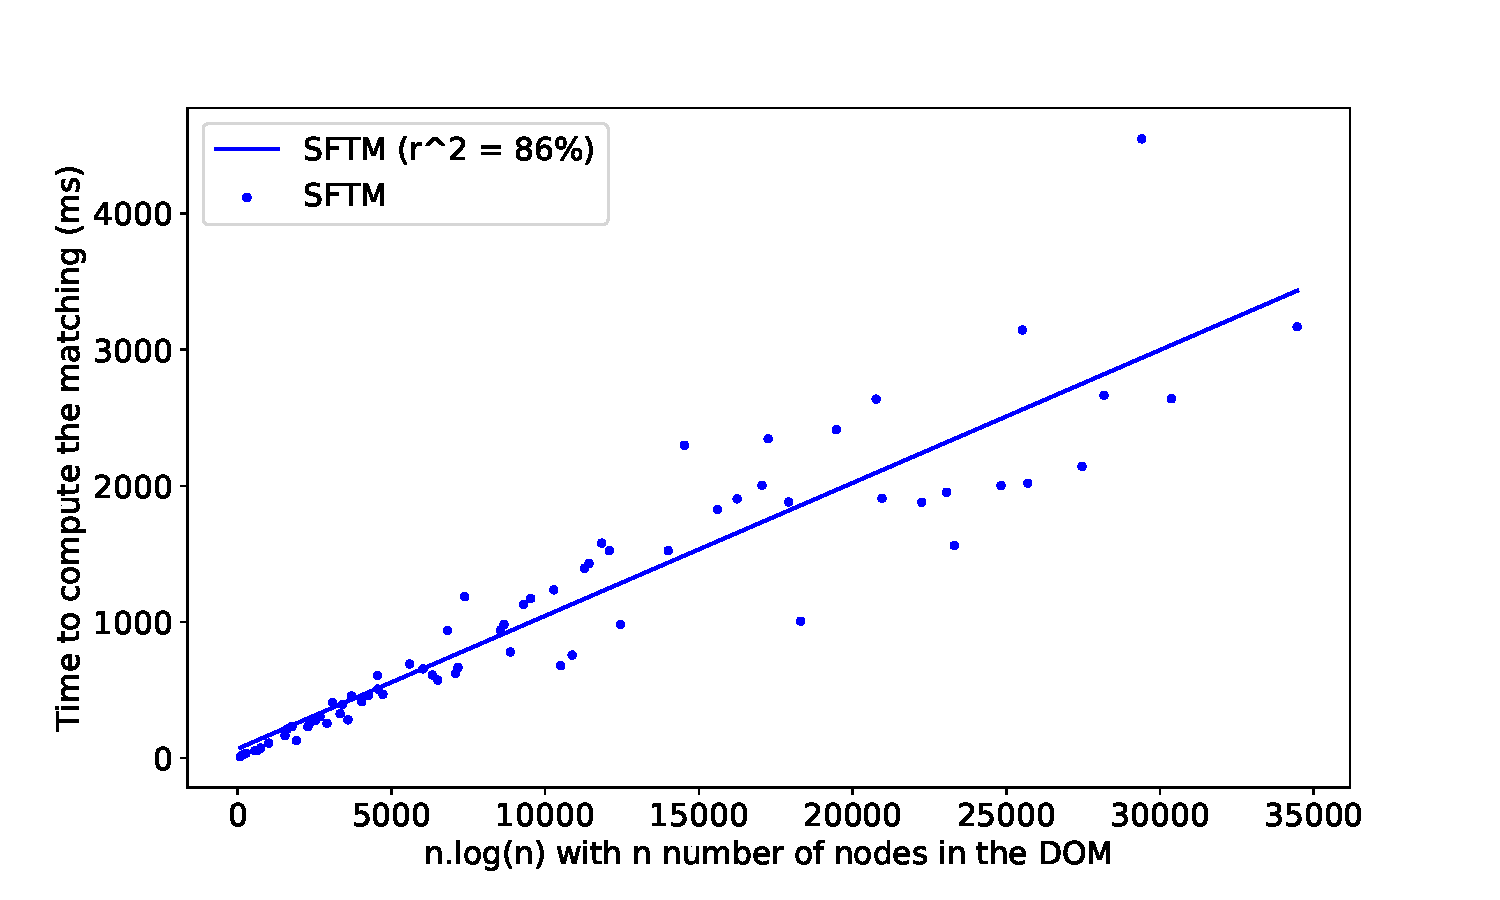
\includegraphics[width=\linewidth]{time_SFTM}
    %     \caption{Average time to compute matching by  $n\ log(n)$ value for SFTM, with $n$ the number of nodes in the DOM}
    %     \label{fig:sftm_speed}
    % \end{figure}
    
% This observation raises the question of the impact of the sublinear threshold function $f$ on the performance of SFTM.
% We therefore conducted a sensitivity analysis of this parameter to better understand potential trade-offs offered by the definition of this function, with regards to the complexity analysis we performed (cf. Section~\ref{sec:complexity}).

\paragraph{Matching efficiency}
The matching efficiency measures how fast a given solution can produce accurate results.
The efficiency is a way to combine both accuracy and speed metrics into one that can be used to compare all solutions.
In our case, we already showed that SFTM outperforms APTED in both accuracy and computation time.
This efficiency measure is thus particularly interesting to compare SFTM to \textsc{XyDiff}, as SFTM outperforms \textsc{XyDiff} in terms of accuracy, but remains slower when it comes to speed.
To compute this matching efficiency, we consider the same metric as~\cite{oliveira2018efficient}---\emph{i.e.}, the number of good matches produced per millisecond.
Figure~\ref{fig:efficiency} reports on the matching efficiency of all three matching solutions.
One can observe that SFTM produces $7.7$ good matches per millisecond on average, which is far above APTED and \textsc{XyDiff} that produce $3.6$ and $2.4$ good matches per millisecond, respectively. 

\begin{figure}
    \centering
    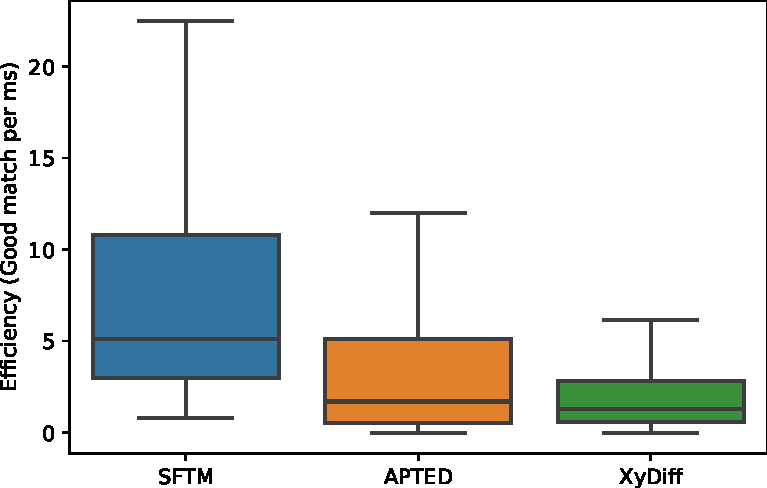
\includegraphics[width=.8\linewidth]{tree-matching/graphs/efficiency}
    \caption{Matching efficiency of SFTM, APTED, and \textsc{XyDiff}.}
    \label{fig:efficiency}
\end{figure}

\paragraph{Parameter sensitivity}
Since we aim at improving the performances of FTM in term of computation times, we study the sensitivity of the sub-linear threshold function $f$, which is a parameter that directly influences the computation time of the algorithm.

Figure~\ref{fig:parameter}, therefore, reports on the evolution of SFTM performances when $f$ varies.
To study the sensitivity of $f$, we choose to use the power function $f(N) = N^\alpha$ as a threshold and display how the computation times and matching accuracy evolve with $\alpha$.

\begin{figure}
    \centering
    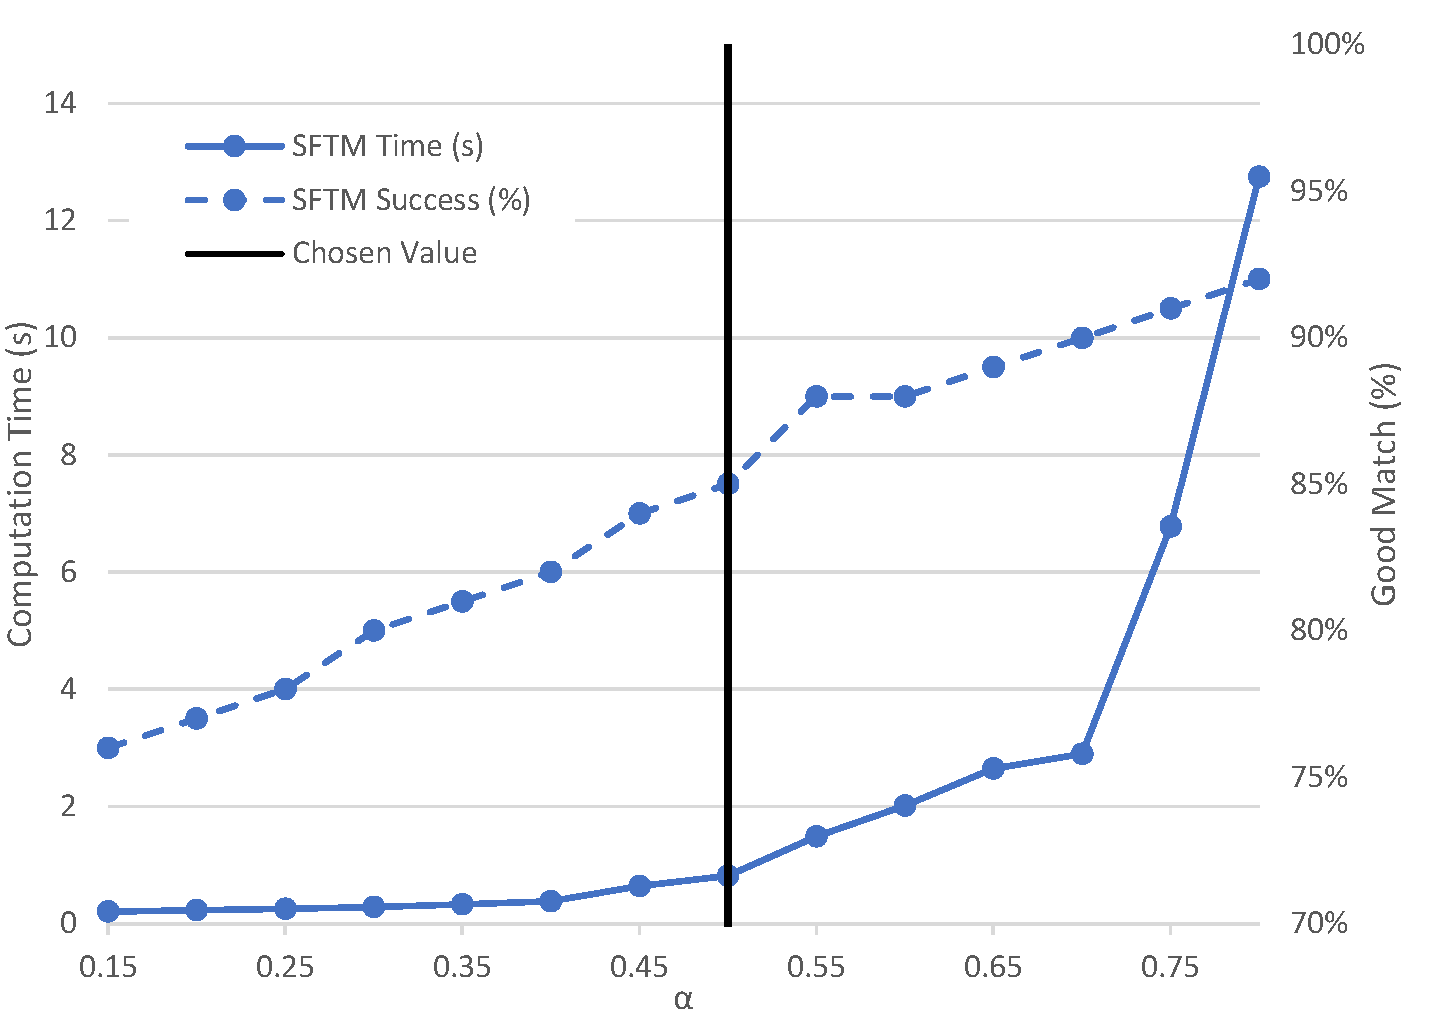
\includegraphics[width=.8\linewidth]{tree-matching/graphs/sensitivity}
    \caption{Performance of SFTM given $f(N) = N^\alpha$ according to $\alpha$.}
    \label{fig:parameter}
\end{figure}

For this experiment, as we are interested in studying the sensitivity of the parameter $\alpha$ on the performances of SFTM, we therefore consider a subset of $243$ pairs from the complete dataset used in previous sections (cf. Section~\ref{sec:performances}), which represents a $6\%$ error margin with $95\%$ confidence.

As expected, when $\alpha$ increases, the quality of the matching and the computation times increase.
However, beyond a certain value of $\alpha$, the increase of computation time is superior to the gain in accuracy: increasing $\alpha$ from $0.5$ to $0.8$ entails more than $10$ times longer computation times for $8\%$ gain in accuracy. 
Intuitively, this is because tokens contained in most nodes provide few relevant information (low IDF), but increase the complexity quadratically.
In this article, we thus adopted $\alpha = 0.5$ (\emph{i.e.}, $f(N) = \sqrt{N}$) as this value achieves good enough performances to demonstrate that SFTM can match two real-life web pages in practical time, with a minimum of compromise on quality.  

\section{Threats to Validity}\label{sec:threats}
The absolute values of completion times depend on the machine on which the algorithms were executed.
As computations took time, we had to run both SFTM, APTED and \textsc{XyDiff} on a server, which is shared among several users.
Although we paid a careful attention to isolate our benchmarks, the available resources of the server might have varied along execution thus impacting our results.
% Nevertheless, the repetition of measures reports a clear signal in favour of SFTM.

Our dataset contains the homepages of the Top\,1k Alexa websites.
The fact that our qualitative evaluation has only been conducted on homepages might have biased the results, as such pages might not be fully representative of the complexity of online documents.
Yet, one can observe that the distribution of page sizes in our datasets offers a good diversity of situations.

The parameters used for SFTM and, in particular, the weights for the propagation may not be optimal.
However, our evaluation shows that the adopted values succeed to report tree matchings that compete with the state-of-the-art accuracy in reasonable times and on a very large variety of web pages, which means the values we provided for the parameters do not require to be tuned for most web pages matching cases.

% Finally, our approach consisting in filtering out the tokens contained by more than $f(N) = \sqrt{N}$ nodes is not backed by any theoretical analysis which means we cannot assure the SFTM algorithm with such tuning will conserve the same performance when the number of nodes grows beyond the empirically studied window.

\section{Conclusion \& Perspectives}\label{sec:conclusion}
Comparing modern real-life web pages is a challenge for which traditional \emph{Tree Edit Distance} (TED) and \textsc{XyDiff} solutions are too restricted and computationally expensive. 
\cite{Kumar2011_FTM} introduced \emph{Flexible Tree Matching} (FTM) to offer a restriction-free matching, but at the cost of prohibitive computational times.

This article thus introduced \emph{Similarity-based Flexible Tree Matching} (SFTM), the first implementation of an advanced \emph{Flexible Tree Matching} (FTM) algorithm with scalable computation times.
We evaluated our solution using mutations on real-life web pages and we showed that SFTM outperforms \textsc{XyDiff} qualitatively and compares to TED, while significantly improving the computation time of the latter.
Our proof of concept demonstrates that accurate matching of real-life web pages in practical time is possible.

Our \textit{label-centric} approach to matching is significantly different than previous \textit{structure-centric} techniques.
In addition to providing a competitive solution to match web pages, we hope that our solution will encourage the development of solutions based on similar approaches.
We also believe that having a robust algorithm to efficiently compare web pages will open up new perspectives within the web community.

In future work, we will further investigate how to improve the quality of the tree matchings by analyzing which situations cause SFTM to report mismatches and to establish guidelines to adjust the exposed parameters.

Finally, whether our work might be applicable to other trees than web DOMs remains to be demonstrated.
Indeed, SFTM strongly relies on the fact that node labels in DOMs are highly differentiating (many specific attributes on each element), which is not the case for all kinds of trees.

%%e.g: Given an element $E$ to locate,  $P$ is an ancestor of $E$, if $P$ has differentiating attributes (like an \textit{id}) we can locate $E$ relatively to $P$ and identify $P$ using its differentiating attributes. 

%\subsubsection{Stateful identification architecture}
%Existing methods to identify elements on a page (xPath) are limited. Notably, they don't allow to express \textit{flexible}, statistics based identifiers. That's why some works have developed some more flexible identification methods [...] and applied them to repair broken locators.

%If we are capable to use more efficient methods than xPath to identify elements as these studies suggest, why use it only to repair locators and not directly as locators?

%In this contribution, we study the problems that moving to such a flexible identification system might rise and suggest a possible architecture allowing to practically use \textit{stateful identification methods}.

% A naive approach would be to sort all edges by increasing cost and select $min(|U|, |V|)$ edges.
% However, doing so would not guarantee to obtain a full matching, since we might have selected several edges linked to the same nodes.
% A valid approach would rather be to: 
% \begin{compactenum}
%     \item Sort all the edges by increasing cost,
%     \item Select the edge $e$ between $u$ and $v$,
%     \item In the ordered list, remove all edges other than $e$ linked to $u$ and $v$,
%     \item Repeat the selection process (from step (2)) until all edges have been selected/
% \end{compactenum}

% While this approach returns a full matching, it only optimizes the decision one-step-ahead.
% In order to approach the optimal matching, we use the same technique as FTM does: the metropolis algorithm~\cite{metropolis1953equation}.
% The metropolis algorithm provides a way to explore a probability distribution by random walking through samples.
% We use this algorithm to random walk through several full matching, and retain the least costly.
% The algorithm needs to be provided with:
% \begin{compactenum}
%     \item An initial sample $M_0$,
%     \item A suggestion function $suggestMatching: M_t \mapsto M_{t+1}$,
%     \item An objective function we want to maximize: $f(M)$,
%     \item A parameter $N$ that defines the number of random walk to perform before returning the best visited sample.
% \end{compactenum}
% Table~\ref{tab:equivalenceMetropolis} shows the equivalence between the general vocabulary and notations commonly used when describing the metropolis algorithm and our specific application to FTM.

% \begin{table}
% \caption{Equivalence between the Metropolis algorithm and FTM}
% \label{tab:equivalenceMetropolis}
% \begin{tabular}{ll}
% \hline
% Metropolis Algorithm & FTM                                    \\
% \hline
% Sample $x$           & Full matching $M$                      \\
% $Q(x_{t+1}|x_t)$     & $suggestMatching: M_t \mapsto M_{t+1}$ \\
% Probability distribution $P(x)$ & $f: M \mapsto \text{quality of } M)$ \\
% \hline
% \end{tabular}
% \end{table}
